% !TEX encoding = UTF-8 Unicode
\documentclass[a4paper]{report}
\usepackage{tikz}
\usepackage[margin=2.5cm]{geometry}
\usepackage{hyperref}
\usepackage{graphicx}
\usepackage{parskip}
\graphicspath{{figures/}{anotherFigureDirectory/}}
\graphicspath{ {./images/} }
\usepackage{listings}
\usepackage{wrapfig}
\usepackage{float}
\usepackage{color}
\usepackage[school,simplified]{pgf-umlcd}
\definecolor{bluekeywords}{rgb}{0.13,0.13,1}
\definecolor{greencomments}{rgb}{0,0.5,0}
\definecolor{turqusnumbers}{rgb}{0.17,0.57,0.69}
\definecolor{redstrings}{rgb}{0.5,0,0}
\definecolor{gray}{rgb}{0.13,0.13,0.13}
\lstdefinelanguage{FSharp}
                {morekeywords={let, new, match, with, rec, open, module,
                namespace, type, of, member, and, for, in, do, begin, end, fun,
                function, try, mutable, if, then, else},
                keywordstyle=\color{bluekeywords},
                sensitive=false,
                numbers=left,  % where to put the line-numbers;(none, left, right)
                numberstyle=\tiny\color{gray},
                morecomment=[l][\color{greencomments}]{///},
                morecomment=[l][\color{greencomments}]{//},
                morecomment=[s][\color{greencomments}]{{(*}{*)}},
                morestring=[b]",
                showstringspaces=false,
                stringstyle=\color{redstrings}
                }

\title{PoP - Ugeopgave 11}
\author{Christoffer, Inge og Pernille}
\date{\today}

\begin{document}
\maketitle
\tikzstyle{block} = [rectangle, draw, fill=blue!20, text centered,
    rounded corners, minimum height=2.5em]
\tikzstyle{cloud} = [rectangle, draw, fill=white, text centered,
    rounded corners, minimum height = 2em]
\tikzstyle{line} = [draw, -latex]



1 Forord
Forordet omhandler selve rapporten. Forordet skal give læseren et billede af rammerne for rapporten.
Forordet indeholder ofte:

\begin{itemize}
\item Hvem har skrevet rapporten, hvornår og i hvilken forbindelse?
\item Hvordan er rapporten blevet til? Er den et eksamensprojekt, er der en opgavestiller og i fald hvem?
Det vil også være naturligt at inkludere en evt. projektkontrakt her, hvis den ikke er lang.
\item Tak til vejledere, faglige hjælpere, og andre, som har bidraget til rapporten.
Forordet er et selvstændigt kapitel i rapporten og i en hvis forstand ikke en del af selve rapporten men
mere et forklæde til rapporten. For korte rapporter er forordet ofte udeladt.
\end{itemize}

VORES EGNE FORORD FRA ISLE ROYALE
\section*{Preface}
As a part of our first semester course in Programming and Problem Solving, we, three budding computer scientists have improved a chess game. We've used the multi paradigm programming language Fsharp (F\#), to code our entire OO environment.

2 Introduktion
Dette afsnit skal give en indledning til rapportens emne på et overordnet plan. Introduktion skal typisk
skrives, så den kan læses sammen med konklusionen med kun et overfladisk kendskab til resten af rapportens indhold. Indledningen indeholder en kort og overordnet introduktion til de faglige elementer, som
rapporten omhandler, motivation for arbejdets udførsel, en kort opsummering af eksisterende arbejde med præcise referencer til litteraturen, og muligvis teasers for de resultater, som er opnået i arbejdet.
Husk at en figur kan være meget illustrativ, når man vil give læseren en overordnet forståelse, se f.eks.
Figur 1.

VORES EGEN INTRODUKTION FRA ISLE ROYALE 
\section*{Introduction}
Isle Royale is a small desolate island located in Lake Superior split by the North America-Canadian border. The island is inhabited by wolves and moose. The population of the two mammals, predator and prey have shown over time to be highly interdependent.
Through no less than 5 decades the research project "Wolves and Moose of Isle Royale" has monitored the lives and deaths of the animals of the island, making \textit{"the longest continuous study of any predator-prey system in the world."}

4 Problemanalyse og design
I dette afsnit beskrives den analyse, som man har gjort for at løse problemet. Det er vigtigt, at de
løsningsmuligheder, der er blevet overvejet, beskrives, samt at man kommer med objektive begrundelser
for de valg, som er gjort. Figurer af f.eks. programdesignet, er som regel at finde i dette afsnit. Dette
afsnit indeholder ofte en overordnet beskrivelse af de centrale datastrukturer samt en skitse af de vigtigste
(dele af) funktioner og deres typer.

\section*{Problem analysis \& design}
The main problem with the improved chess game was to make sure that the king could not move to a square that was an available move for an opponent piece. We considered many approaches to solve this problem.
Our first approach was to use the already implemented functionality of the getVacantNNeighbours, which returned a list of available moves and which opponent pieces that could be killed in a move. We
would then use this list og available kills to check if an available move would cause an opponent piece to have a king as a kill. We decided not to do this as it was going to slow down the game. We decided to
check if the kings available moves were the same as the opponent kings available moves and if they are we then removed them as available moves. To check if there was a collision of the available moves with the rook we
decided to check if one of the coordinates of the kings avialable moves was also one of the coordinates of the rook.
DET HAR VI IKKE VÆRET SUPER GODE TIL AT SKRIVE TIDLIGERE, VI HAR SLET IKKE TIDLIGERE SKREVET OM LØSNINGSMULIGHEDER, SÅ DET TÆNKER JEG ER DET VI FOKUSERER PÅ AT SKRIVE LIDT OM.



5 Programbeskrivelse
Programbeskrivelsen er en gennemgang af det producerede program, dvs. en gennemgang af de centrale
problemstillinger med at omforme centrale valg for Problemanalysen til det konkrete program. Det vil
ofte være naturligt kun at fokusere på ikke-oplagte løsninger og særlige indsigter og tricks, der er brugt.
Eksempelvis kunne man inkludere programkode stumper som f.eks. vist i Figur 2
Programbeskrivelsen giver en kort beskrivelse af, hvordan programmet bruges. F.eks. hvis programmet
skal køres fra kommandolinjen, hvilke argumenter, der kan benyttes, og hvad er deres effekt.

\section*{Program description}

DET HER AFSNIT TÆNKER JEG PRIMÆRT BARE SKAL BESTÅ I UML'EN NEDENFOR OG SÅ LIDT INDLEDENDE TEKSTFYLD, DER ARBEJDER SIG FREM TIL AT PRÆSENTERE UML'EN.

\subsection*{UML}
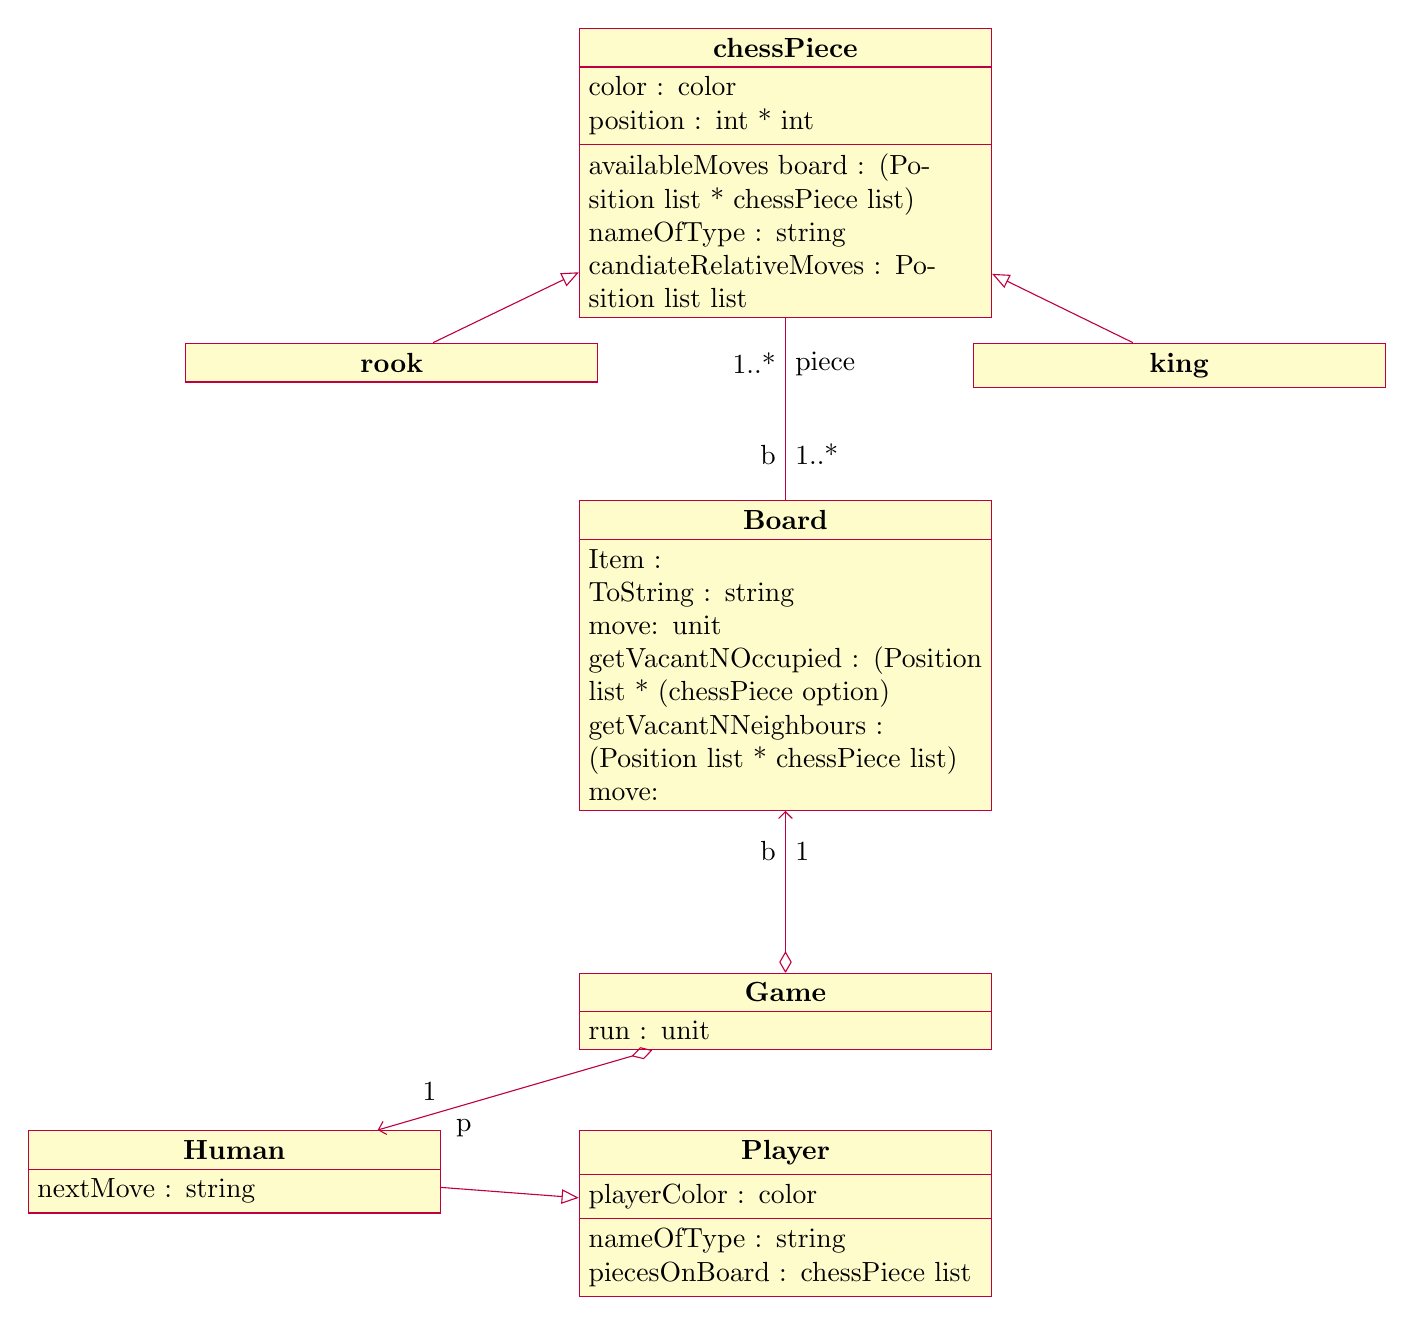
\begin{tikzpicture}
 \begin{class}[text width=5cm]{chessPiece}{0,0}
  \attribute{color : color}
  \attribute{position : int * int}
  \operation{availableMoves board : (Position list * chessPiece list)}
  \operation{nameOfType : string}
  \operation{candiateRelativeMoves : Position list list}
 \end{class}
 \begin{class}[text width=5cm]{rook}{-5,-4}
  \inherit{chessPiece}
 \end{class}
 \begin{class}[text width=5cm]{king}{5,-4}
  \inherit{chessPiece}
 \end{class}
 \begin{class}[text width=5cm]{Board}{0,-6}
  \operation{Item : }
  \operation{ToString : string}
  \operation{move: unit}
  \operation{getVacantNOccupied : (Position list * (chessPiece option)}
  \operation{getVacantNNeighbours : (Position list * chessPiece list)}
  \operation{move: }
 \end{class}
 \association{Board}{b}{1..*}{chessPiece}{1..*}{piece}
 \begin{class}[text width=5cm]{Game}{0,-12}
  \operation{run : unit}
 \end{class}
 \aggregation{Game}{b}{1}{Board}
 \begin{class}[text width=5cm]{Player}{0,-14}
  \attribute{playerColor : color}
  \operation{nameOfType : string}
  \operation{piecesOnBoard : chessPiece list}
 \end{class}
  \begin{class}[text width=5cm]{Human}{-7,-14}
  \inherit{Player}
  \operation{nextMove : string}
 \end{class}
 \aggregation{Game}{p}{1}{Human}
\end{tikzpicture}



\end{document}